\documentclass{beamer}
\usepackage{ dsfont }
\usepackage[utf8]{inputenc}
\usepackage[english]{babel}
\setbeamersize{text margin left=10pt, text margin right=10pt} %new code
\usepackage{graphicx}
\usepackage{float}
\usepackage{subcaption}

\usepackage{animate}
\usepackage{movie15}
\usepackage{breqn, bm}
\usepackage{tcolorbox, amsmath}
\usepackage{subcaption}

\definecolor{notgreen}{RGB}{255,127,0}
\definecolor{green}{RGB}{49,150,3}
\setbeamerfont{headline}{size=\small}


%----------------------------------------------------------------------------------------
%	 Package
%----------------------------------------------------------------------------------------
\usepackage{color}
\usepackage{url}
\beamertemplatenavigationsymbolsempty
\definecolor{cadmiumred}{rgb}{0.8, 0.8, 0.8}

%----------------------------------------------------------------------------------------
%	 Presentation settings
%----------------------------------------------------------------------------------------

\usetheme{Madrid}
\usecolortheme{beaver}

\setbeamertemplate{itemize items}[triangle] 
\setbeamertemplate{enumerate items}[default]
 
\title[Variational Drop Out]{
	Seminar: Practical Machine Learning \\ 
	\vspace{1cm}
	\textbf{\textcolor{black}{Variational Drop Out}}}

\author{Ashuha Arseniy}
\institute[MIPT]{
	Yandex, Moscow Institute of Physics and Technology\\
	
	\medskip
	
	\href{mailto:ars.ashuha@gmail.com}{\nolinkurl{ars.ashuha@gmail.com}}}

\date{\today}

\newcommand{\Expect}{\mathsf{E}}
\newcommand{\MExpect}{\mathsf{M}}
\newcommand{\cov}{\mathsf{cov}}
\setbeamertemplate{section in toc}[circle]


\begin{document}
\begin{frame}
	\titlepage 
	\footnotesize{ \emph{Kingma, et al. "Variational Dropout and the Local Re-parameterization Trick." NIPS'15}}
\end{frame}

\begin{frame}{Binary  Drop Out}
		 Dropout is a technique for regularization of neural network
		
		$$
			B = (A \circ \xi) \theta
		$$
		
		\begin{center}
			$A$ -- inputs, $\xi \thicksim Bernulli(1-p)$,  $\theta$ -- weights, $B$ -- outputs
		\end{center}
		
		\begin{center}
			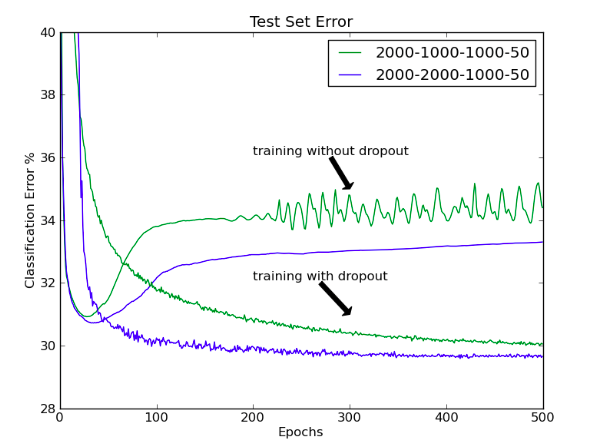
\includegraphics[scale=0.3]{img/binary}
		\end{center}
		
		
		\vspace{-0.5cm}
		
		\noindent\rule{12cm}{0.4pt}
		\footnotesize{ Hinton at el.: Improving neural networks by preventing co-adaptation}
\end{frame}
	
\begin{frame}{Gaussian  Drop Out}
	$$B = (A \circ \xi) \theta, \xi \thicksim Bernulli(1-p)$$
			
	\begin{itemize}
		\item During dropout testing we need to scale the weights on $$\theta_{test} = 1/(1 - p)\theta_{train}$$
		
		\item The same can be achieved by scale activation on $1/(1 - p)$ at training
			$$B = (A \circ \xi) \theta~~~~~\rightarrow~~~~~B = (A \circ \xi/(1-p))  \theta$$ 
			
			$$\mathds{E}[\xi_{ij}/(1-p)] = 1, Var[\xi_{ij}/(1-p)] = p/(1-p)$$
		
		\item Using a distribution with the same mean and variance, works as well
	\end{itemize}
	
	\begin{center}
		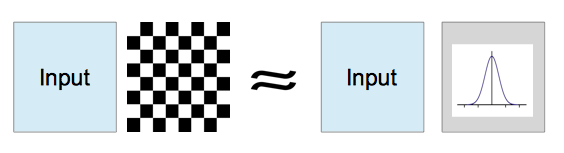
\includegraphics[scale=0.4]{img/gaus}
	\end{center}
	
	\vspace{-0.2cm}
	
	
	\noindent\rule{12cm}{0.4pt}
	\footnotesize{Srivastava at el.: A Simple Way to Prevent Neural Networks from Overfitting}

\end{frame}
	
\begin{frame}{Fast Gaussian  Drop Out}  
	Gaussian dropout:
	\vspace{-1.5cm}
	\begin{center}
		 $$B = (A \circ \xi) \theta$$
		$A$ -- input matrix, $\xi \thicksim N(1, \alpha)$, $\theta$ -- weight matrix, $B$ -- output matrix
	\end{center}
	
	\begin{itemize}
		\item It means that activation also distributed Normal
		
		$$q(b_{mj} | A, \theta, \alpha) = N(\gamma_{mj}, \delta_{mj})~~~\gamma_{mj} = \sum_i a_{mi}\theta_{ij}, \delta_{mj} = \alpha \sum_i a_{mi}^2\theta_{ij}^2$$
	\end{itemize}
	
	\begin{center}
		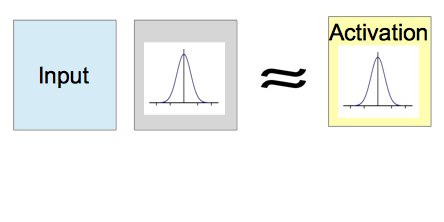
\includegraphics[scale=0.4]{img/act}
		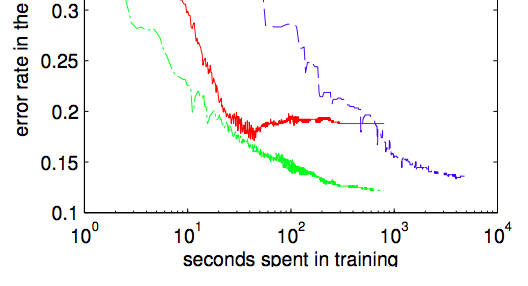
\includegraphics[scale=0.3]{img/fast}
	\end{center}
	
	\vspace{-0.6cm}
		
		\begin{itemize}
			\item It's equivalent Normal distribution on weight $q(w_{ij}) = N(\theta_{ij}, \alpha\theta_{ij}^2)$
			
			\begin{center}
				$b_{ij} =  \sum_k a_{ik}(1+\sqrt{alpha}\cdot\epsilon)\theta_{kj},~~~\epsilon \thicksim N(0, 1),  N(\mu, \sigma^2) = \mu + \sigma\epsilon$
			\end{center}
		\end{itemize}
		
	\vspace{-0.2cm}
	
	\noindent\rule{12cm}{0.4pt}
	\footnotesize{ Wang at el.: Fast dropout training}
\end{frame}

\begin{frame}{Mind Summary}
	\begin{itemize}
		\item We transform $\alpha$ from hyper-parameter to parameter
		\item Also transform model to probabilistic  
		\item We want to use stochastic variational toolbox 
		\item Our goal is to see that dropout  is special case of Bayesian Inference
	\end{itemize}

\end{frame}


\begin{frame}{Variational Lower Bound}
	
	We want to determinate parameters $\phi = (\theta, \alpha)$ of distribution on $Z=w_{ij}$
	\vspace{0.2cm}
	
	 Let's use Bayesian  toolbox:
	\begin{enumerate}
		 \item Defined $p(X, Z)$, $X$ -- observed variables, $Z$ -- hidden variables 
		 \item We want to find $p(Z|X) = P(X, Z) / P(X)$, $P(X)$ usually intractable 
		 \item Therefor we will try to approximate $p(Z|X) \approx q_\phi(Z)$
		 \item Derive Variational Lower Bound		 
	\end{enumerate}
			\begin{center}
			 $log~P(X) =  \int q_\phi(Z) log~P(X) dZ =$  
			 $\int log~\frac{p(X, Z)q_\phi(Z)}{p(Z|X)q_\phi(Z)}~q_\phi(Z) dZ = $ 
			
			 $\int log~\frac{p(X, Z)}{q_\phi(Z)}~q_\phi(Z) dZ  + \int log~\frac{q_\phi(Z)}{p(Z|X)}~q_\phi(Z) dZ = $
			\vspace{0.2cm}
			
			 $= \mathcal{L}(q_\phi(Z), p(X, Z)) +  D_{KL}(q_\phi(Z), p(Z|X))$
			\end{center}
			
	
	\vspace{-0.4cm}
	
	\begin{enumerate}
		\item[5.] ~~~~~~~~~~~$\mathcal{L} = \mathds{E}_{q_\phi(Z)} log~p(X|Z) - D_{KL}(q_\phi(Z), p_{prior}(Z))$
	\end{enumerate}
	
	~~~~~~~~~~~~~~~~~~~~~~~~\textcolor{red}{likelihood expectation}~~~~~~~	\textcolor{green}{regularizer}
\end{frame}

\begin{frame}{Stochastic Gradient Variational Lower Bound}	
	$$\mathcal{L} = \mathds{E}_{q_\phi(Z)} log~p(X|Z) - D_{KL}(q_\phi(Z), p_{prior}(Z))$$
	
	\begin{enumerate}
		\item We cant take gradient by parameters by Naive way
		\item The problem is in estimate this derivative 
			$$\frac{\partial}{\partial \phi}\mathds{E}_{q_\phi(Z)} log~p(X|Z) \neq \mathds{E}_{q_\phi(Z)} \frac{\partial}{\partial \phi} log~p(X|Z)$$
		\item Lets use  re-parametrization trick:
		$$\frac{\partial}{\partial \phi}\mathds{E}_{q_\phi(Z)} log~p(X|Z) = \mathds{E}_{N(\epsilon|0, 1)} \frac{\partial}{\partial \phi} log~p(X|Z=f(\epsilon, \phi))$$
		\item Example:
		$$f(\epsilon, (\theta, \alpha)) = \theta + \sqrt{\alpha}\theta\epsilon$$
	\end{enumerate}
	
	\noindent\rule{12cm}{0.4pt}
	\footnotesize{ Kingma, et al. "Auto-Encoding Variational Bayes" }
\end{frame}

\begin{frame}{Variational Drop Out}	
	\begin{enumerate}
		 \item During dropout training we optimize Expectation on MLE
			$$\mathds{E}_{q_{\alpha, \theta}}log~p(X| \alpha, \theta) \rightarrow \max_\theta$$
		\vspace{-0.5cm}
		 \item During dropout training we optimize VLB with fixed $\alpha$, $\alpha=constant$
		 $$\mathds{E}_{q_{\alpha, \theta}}log~p(X| \alpha, \theta) + D_{KL}(\alpha) \rightarrow \max_{\theta, \alpha}$$ 
		
		\vspace{-0.5cm}
		 $$\mathcal{L} = \mathds{E}_{q_\phi(Z)} log~p(X|Z) - D_{KL}(q_\phi(Z), p_{prior}(Z))$$
		
		
		 \item There exist the $p(log(|w_{ij}|)) \propto c$ prior satisfy this conditions  
		 \item Prior interpretation -- number of significant digits
	\end{enumerate}
	
	\vspace{0.2cm}
	 We can train personal alpha for: weight, features, layer
	\begin{itemize}
		 \item Uncorrelated -- separate alpha per weight
		 \item Correlated  -- separate alpha per weight correspond to same features
		
			$$q(Z) = q(w_{ij}) = N(\theta_{ij}, \alpha_{ij}\theta_{ij}^2)~or~N(\theta_{ij}, \alpha_{i}\theta_{ij}^2)$$
	\end{itemize}
	
	\noindent\rule{12cm}{0.4pt}
	\footnotesize{ Kingma, et al. "Variational Dropout and the Local Reparameterization Trick" }
\end{frame}

\begin{frame}{Examples}
	\begin{enumerate}
		\item MNIST
			\begin{center}
				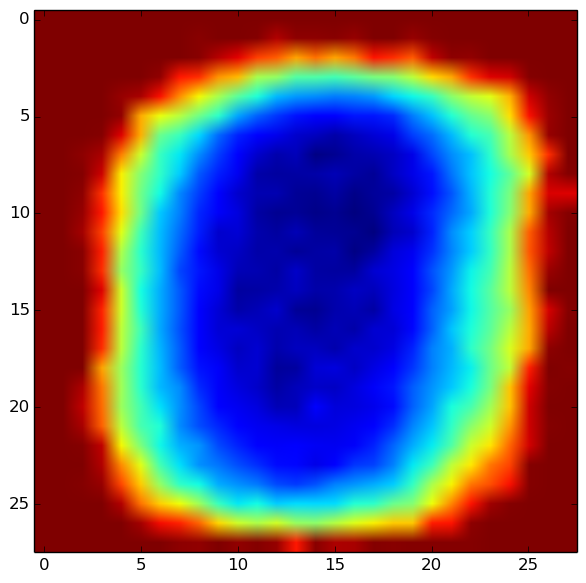
\includegraphics[scale=0.18]{img/mnist_reg}
				
\includegraphics[scale=0.2]{img/mnist}
			\end{center}
		\item CIFAR
			\begin{center}
				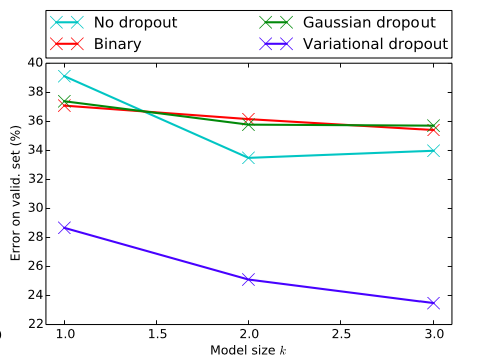
\includegraphics[scale=0.3]{img/cifar}
			\end{center}
	\end{enumerate}
\end{frame}

\begin{frame}{Summary}
	\begin{itemize}
		\item Bernoulli dropout can be transform to Gaussian with same E, Var
		\item Gaussian input noise equal Gaussian weight noise  
		\item Reinterpretation weight Gaussian noise as posterior distribution
		\item Show that dropout training is special case of Bayesian Inference
		\item Offered efficient low variance gradient estimator  
	\end{itemize}
\end{frame}

\end{document}

